\documentclass[pra,
aps,
twocolumn,
superscriptaddress,
groupedaddress,
nofootinbib,
reprint
]{revtex4-1}

% PACKAGES
\usepackage{amsmath,amsfonts, amssymb, amsthm}
\usepackage{bm, bbm, physics, mathtools}
\usepackage{graphicx, subfigure}
\usepackage{xcolor, enumerate}
\usepackage{xifthen, hyperref}
\usepackage[capitalise]{cleveref}

\hypersetup{
	colorlinks=true,  
	linkcolor=blue,   
	citecolor=blue,   
	urlcolor=blue     
}

\newcommand{\crefrangeconjunction}{--}
\creflabelformat{figure}{(#2#1#3)}

% COMMENT NOTATION
\newcommand{\nick}[1]{{\color{red}#1}}
\newcommand{\ddd}[1]{\textcolor{blue}{#1}}

% ENVIRONMENTS
\newtheorem{theorem}{Theorem}
\newtheorem{proposition}[theorem]{Proposition}
\newtheorem{lemma}[theorem]{Lemma}
\newtheorem{definition}[theorem]{Definition}

% REFERENCES
\iffalse
\renewcommand{\eqref}[1]{Eq.~(\ref{#1})}
\newcommand{\figref}[1]{Fig.~(\ref{#1})}
\newcommand{\tabref}[1]{Tab.~(\ref{#1})}
\newcommand{\secref}[1]{Section~(\ref{#1})}
\newcommand{\appref}[1]{Appendix~(\ref{#1})}
\newcommand{\defref}[1]{Definition~\ref{#1}}
\newcommand{\lemref}[1]{Lemma~\ref{#1}}
\newcommand{\thmref}[1]{Theorem~\ref{#1}}
\fi

% SYMBOL DEFINITIONS
\renewcommand{\cal}[1]{\mathcal{#1}}

\newcommand{\reals}{\mathbb{R}}
\newcommand{\id}{\mathbbm{1}}
\newcommand{\idc}{1_{\rm{C}}}
\newcommand{\supf}{\mathfrak{c}}
\renewcommand{\tr}{{\rm{tr}}}
\renewcommand{\det}{{\rm{det}}}
\newcommand{\floor}[1]{\left\lfloor #1 \right\rfloor}
\newcommand{\ent}[2]{S\left( #1 \middle\vert\middle\vert #2 \right)}
\newcommand{\ents}{{\ent{\frac{m}{n}}{p}}}

\def\dummy{\ell}
\def\NN{n}
\def\mmf{i}
\def\nnf{n}
\def\mlt{m}
\def\ii{i}
\def\jj{j}
\def\kk{k}
\def\II{I}
\def\nn{n}
\def\tt{n'}
\def\mm{a}
\def\wp{u}
\def\wn{v}

\newcommand{\too}[1]{^{\otimes #1}}
\newcommand{\noisys}{\rho_{\rm{S}}}
\newcommand{\noisysn}{\rho_{\rm{S}}(\epsilon)^{\otimes \nn}}
\newcommand{\noisysN}{\rho_{\rm{S}}(\epsilon)^{\otimes \NN}}

\newcommand{\spanv}[1]{
    {{\rm{span}}\left\{#1\right\}}
}
\newcommand{\conv}[1]{
    {{\rm{conv}}#1}
}
\newcommand{\orb}[1]{
    {{\rm{orb}}(#1)}
}
\newcommand{\sn}[1]{
    {{\rm{sn}}\left(#1\right)}
}
\newcommand{\mana}[1]{
    {{\rm{mana}}\left(#1\right)}
}
\newcommand{\lc}[2]{
	{{\rm{L}}_{#1|#2}}
}

\newcommand{\bmx}{\bm{x}}
\newcommand{\bmy}{\bm{y}}
\newcommand{\bmz}{\bm{z}}
\newcommand{\bmu}{\bm{u}}
\newcommand{\bmw}{\bm{w}}
\newcommand{\bmo}{\bm{0}}
\newcommand{\bmd}{\bm{d}}
\newcommand{\bma}{\bm{a}}
\newcommand{\bmxi}{\bm{\xi}}
\newcommand{\bmg}{\bm{g}}

\newcommand{\zd}[1][]{
    \ifthenelse{\isempty{#1}}{
    {\mathbb{Z}_d} }{
    {\mathbb{Z}_{#1}}}
}
\newcommand{\hd}[1][]{
    \ifthenelse{\isempty{#1}}{
    {\cal{H}_d} }{
    {\cal{H}_{#1}}}
}
\newcommand{\pd}[1][]{
    \ifthenelse{\isempty{#1}}{
    {\cal{P}_d} }{
    {\cal{P}_{#1}}}
}
\newcommand{\cd}[1][]{
    \ifthenelse{\isempty{#1}}{
    {\cal{C}_d} }{
    {\cal{C}_{#1}}}
}
\newcommand{\spd}[1][]{
    \ifthenelse{\isempty{#1}}{
    {{\rm{Sp}}(2, \zd)} }{
    {{\rm{Sp}}(2, \zd[#1])}}
}
\newcommand{\gp}[1][]{
    \ifthenelse{\isempty{#1}}{
    {\rm{GP}_d} }{
    {\rm{GP}_{#1}}}
}
\newcommand{\stoch}[1][]{
    \ifthenelse{\isempty{#1}}{
    {{\rm{S}}_d(\bmd)} }{
    {{\rm{S}}_d(#1)}}
}
\newcommand{\stochw}[1][]{
    \ifthenelse{\isempty{#1}}{
    {{\rm{S}}_{d^2}(\W{\sigma})} }{
    {{\rm{S}}_{d^2}(#1)}}
}
\makeatletter
\def\W{\@ifnextchar[{\@with}{\@without}}
\def\@with[#1]#2{ 
    {{\rm{W}}_{#2}\left(#1\right)} }
\def\@without#1{ 
    {{\rm{W}}_{#1}} }
\makeatother

\newcommand{\T}{\cal{T}}
\newcommand{\Z}{\cal{Z}}

\newcommand{\C}{\cal{C}}
\newcommand{\E}{\cal{E}}
\newcommand{\J}{\cal{J}}
\newcommand{\R}{\cal{R}}
\newcommand{\D}{\cal{D}}
\newcommand{\F}{\cal{F}}
\renewcommand{\O}{\cal{O}}
\newcommand{\M}{\cal{M}}

\newcommand{\Fmax}{\F_{\rm{max}}}
\newcommand{\Omax}{\O_{\rm{}max}}
\newcommand{\Rmax}{\R_{\rm{}max}}
\newcommand{\Pis}{\Pi_{\rm{s}}}
\newcommand{\Pio}{\Pi_{\rm{o}}}

\newcommand{\cptp}{{\rm{CPTP}}}
\newcommand{\cpos}{{\rm{CP}}}
\newcommand{\so}{{\rm{SO}}}
\newcommand{\stab}{{\rm{STAB}}}
\newcommand{\spo}{{\rm{SPO}}}
\newcommand{\cspo}{{\rm{CSPO}}}
\newcommand{\rcu}{{\rm{RCU}}}
\newcommand{\tho}{{\rm{TO}}}
\newcommand{\cpwp}{{\rm{CPWPO}}}
\newcommand{\ru}{{\rm{RU}}}


\begin{document}

\begin{abstract}
Magic states are essential for achieving universality in fault-tolerant schemes.
Magic resource theories attempt to quantify magic via monotones and thus describe the manipulation of magic states.
Here we introduce the concept of majorization fragments as a more generalised projection of such theories in discrete odd dimensions which allows for more powerful results than what monotones can provide.
Fragments naturally link the symmetries of a gate sequence with conditions on the convertibility between states.
We demonstrate the power of fragments by providing exact conditions for the convertibility of single-copy qutrit magic states as well as stricter distillation bounds than the established mana monotone in any odd dimension.
\end{abstract}

\preprint{APS/123-QED}

\title{Majorization Fragments in Resource Theories of Magic}

\author{Nikolaos Koukoulekidis}
	\affiliation{Department of Physics, Imperial College London, London SW7 2AZ, UK}
	\email{nk2314@imperial.ac.uk}
\author{David Jennings}
	\affiliation{School of Physics and Astronomy, University of Leeds, Leeds, LS2 9JT, UK}
	\affiliation{Department of Physics, Imperial College London, London SW7 2AZ, UK}

\date{\today}
\maketitle

%%%%%%%%%%%%%%%%%%%%%%%%%%%%%%%%%%%%%%%%

\section{Introduction}
\label{sec:intro}

\begin{enumerate}
    \item Fault-tolerance~\cite{cit:raussendorf, cit:gross2, cit:markov, cit:gross, cit:nest, cit:nest2, cit:vidal, cit:fujii, cit:gottesman}
    \item Magic~\cite{cit:veitch, cit:veitch2, cit:wang, cit:wang2, cit:howard, cit:campbell, cit:gross3, cit:gross4}
    \item Bringing in majorization~\cite{cit:cwiklinski, cit:lostaglio2, cit:lostaglio, cit:gour, cit:janzing, cit:brandao2, cit:gour2, cit:marshall, cit:nielsen}
    \item Section breakdown
\end{enumerate}

%%%%%%%%%%%%%%%%%%%%%%%%%%%%%%%%%%%%%%%%

\section{Magic Resource Theories}
\label{sec:magic}

\subsection{Introduction}

Magic states are necessary for achieving universal quantum computation within fault-tolerant schemes.
Identifying magic as a resource for quantum universality has led to several theories which try to provide a framework for its quantification and manipulation \nick{CITE}.
The main question that such a theory attempts to answer is:
\begin{center}
    \emph{Given two magic states $\rho$ and $\rho'$ is there a free operation that can convert $\rho$ to $\rho'$?}
\end{center}

We are interested in all resource theories of magic $\R = (\F, \O)$ in which free operations cannot generate any amount of resource. 
Further denote by $\D$ the set of states considered under the theory, that is the union of free and resource states.
The structure of such theory is described by a partial order \nick{CITE}, hereinafter called a \emph{pre-order}, $\prec_{\R}$ between states.
We write $\rho' \prec_{\R} \rho$ iff there exists $\E \in \O$ such that $\E(\rho) = \rho'$.
Naturally, states may be incomparable under the given theory, meaning that there exists no free operation that converts one to the other.
We further call $\R' = (\F', \O')$ a \emph{subtheory} of $\R$ iff $\F' \subseteq \F$ and $\O' \subseteq \O$. 
The above notation will be used for general resource theories as well.

Formally, the no resource generation condition on the theories translates into two assumptions:
\begin{enumerate}[I]
    \item Free operations send free states into free states, $\E: \F \mapsto \F$, for all $\E \in \O$;
    \item Resource theory $\R$ is a completely free state preserving theory, in the sense that for any $d$-dimensional ancilla system and all free operations $\E$, $(\id_d \otimes \E ) \sigma \in \F$ whenever $\sigma \in \F$.
\end{enumerate}
The first assumption simply states that resources cannot be generated for free and is a minimal requirement for a resource theory. 
An immediate consequence is that if statistical mixing is included in $\O$, then the resource theory is convex.
Convex resource theories have attracted a lot of attention recently \nick{CITE} and include the magic theories discussed in~\cref{sec:prev}.
The second assumption implies that resources cannot be generated even when ancillas are allowed \nick{example of T state generation on Bell state by Campbell}.

Monotones are often used \nick{CITE} to address the question of state convertibility, although such approaches are usually generic.
A monotone of any general resource theory is a projection of the theory onto the non-negative real numbers, collapsing the pre-order of the theory to the total order defined on the real line.
This is the \nick{most naive} non-trivial projection under which the images of incomparable states can be compared.
Our first contribution is the introduction of a generalised notion of \emph{resource projection} which maps a general resource theory onto a subtheory which in principle still retains a partial structure.
Applying this notion on existing magic theories highlights the hidden stochasticity that governs magic state conversions.
We show that a magic theory can be subdivided into \emph{fragments} \nick{expand}

\subsection{Previous work}\label{sec:prev}

The stabilizer theory \nick{CITE} is the first theory to introduce the idea of magic and it is discussed in sufficient detail for our purposes in~\cref{sec:so}. 
It comprises of the so-called ``stabilizer'' states ($\stab$) and operations ($\so$), while non-stabilizer (resource) states are called magic.
The stabilizer operations can be expressed in terms of a Stinespring dilation as 
\begin{equation}
    \E(\rho) = \tr_E [U(\rho \otimes \sigma_E)U^\dagger],
\end{equation} 
for an ancilla stabilizer state $\sigma_E$. 
The motivation of the theory stems from the fact that stabilizer operations are experimentally straightforward to implement and they can be used to detect and correct errors on the stabilizer states due to their construction \nick{CITE}.
The Gottesman-Knill theorem however indicates that stabilizer operations need to be supplemented with magic states in order to achieve universality, justifying the term ``magic''.

Generalisations of the stabilizer theory appear in the literature intending to include broader classes of operations \nick{CITE}.
The class of stabilizer preserving operations ($\spo$) is defined as the set of $\cptp$ maps that send stabilizer states into stabilizer states~\cite{cit:ahmadi}.
An important subclass of $\spo$ is the set of completely stabilizer preserving operations ($\cspo$), which intuitively cannot induce ``non-stabilizerness'' even when applied to only part of a quantum state, i.e. operations $\E$ such that $(\id_d \otimes \E ) \sigma \in \stab$ for all positive dimensions $d$ whenever $\sigma \in \stab$.

Even though non-stabilizerness is a necessary resource for universality, it has been proven insufficient for magic state distillation~\cite{cit:bravyi, cit:campbell}.
In fact, all states with non-negative Wigner distributions have been proven to be efficiently classically simulable in~\cite{cit:mari}, a result that serves as a generalization of the Gottesman-Knill theorem.
The Wigner distribution of a state in odd prime dimensions is discussed rigorously in~\cref{sec:wigner} and arises as the unique quasi-probability representation of quantum theory that identifies non-contextuality exactly with the states that are efficiently classically simulable~\cite{cit:howard2, cit:veitch2}.
In this framework, the stabilizer states are the only pure states represented with non-negative distributions~\cite{cit:gross3}. 
However, there exist mixed states with non-negative Wigner distributions that are not mixtures of stabilizer states~\cite{cit:gross}.
Therefore, stabilizer-preserving theories have been extended to a theory that preserves state ``Wigner positivity''~\cite{cit:wang}, formally defined in~\cref{sec:wigner} for odd prime dimensions.
Informally, it can be considered as the maximal theory of magic $\Rmax = (\Fmax, \Omax)$, where free states have non-negative Wigner distributions and free operations completely preserve this property.

\ddd{[Things we must emphasize:
\begin{enumerate}
\item We can tackle more `physicsy' questions like: how much magic can be distilled via free operations with some given fixed-point structure? E.g. 
\item This allows a diagnostic on the kind of operations needed to do good distillation. I.e. what fixed point structure should they have?
\item We go beyond magic monotones and replace a monotone with a $\sigma$-fragment.
\item We can get both upper and lower bounds on magic distillation.
\end{enumerate}•
}
%%%%%%%%%%%%%%%%%%%%%%%%%%%%%%%%%%%%%%%%

\section{Phase Space formalism}
\label{sec:ps}

\subsection{Stabilizer Theory}\label{sec:so}

Let $\{\ket{k}\}_{k \in \zd}$ be the standard computational basis for an arbitrary fault-tolerant scheme, defined over the finite field $\zd = \{ 0, 1, \dots,d-1 \}$, with $d$ an odd prime. 
Since the field has character $d$, addition and multiplication on the field are always considered modulo $d$.
The Hilbert space of any system associated with this scheme is $\hd \coloneqq \spanv{\ket{k}: k \in \zd}$.

The generalised Pauli matrices $X, Z$ can be defined by their respective roles as shift and phase operators,
\begin{align}
    X \ket{k} &= \ket{k + 1} \label{eq:xpauli}\\
	Z \ket{k} &= \omega^k \ket{k}, \label{eq:zpauli}
\end{align}
where $\omega \coloneqq e^{2\pi i/d}$ is the $d$-th root of unity. 

The Hilbert space $\hd$ is associated with a phase space $\pd \coloneqq \zd \times \zd$, where every point $\bmx \coloneqq (x_0, x_1)$ corresponds to a displacement operator, defined as
\begin{equation}\label{eq:ddef}
    D_{\bmx} \coloneqq \tau^{x_0 x_1} X^{x_0} Z^{x_1},\ \bmx  \in \pd.
\end{equation}
The phase factor $\tau \coloneqq -\omega^{1/2}$ ensures unitarity.
For a system with composite Hilbert space, $\hd = \hd[d_A] \otimes \hd[d_B]$, the displacement operators are defined as
\begin{equation}\label{eq:composited}
    D_{\bmx_A \oplus \bmx_B} \coloneqq D_{\bmx_A} \otimes D_{\bmx_B},
\end{equation}
where $\bmx_A \oplus \bmx_B \coloneqq (x_{A0}, x_{B0}, x_{A1}, x_{B1}) \in \pd[d_A] \times \pd[d_B]$.

The displacement operators, form a group under matrix multiplication modulo phases,
\begin{equation}\label{eq:gp}
    \gp \coloneqq \{ \tau^k D_{\bmz}: k \in \zd, \bmz \in \pd\}.
\end{equation}
The Clifford unitaries $\cd$ can then be defined as the normaliser of this group, \nick{Reformulate for copies of qudits: $\gp,\ \cd \rightarrow \gp^n,\ \cd^n$. $C-SUM$s live in $\cd^2$}
\begin{equation}
    \cd \coloneqq \{ U \in {\rm{SU}}(d): U\gp U^\dagger = \gp \}.
\end{equation}
The pure stabilizer states are then the orbit of the Clifford unitaries over a computational basis state,
\begin{equation}\label{eq:stab}
    \stab_{{\rm{pure}}} \coloneqq \{ U\ketbra{0}{0}U^\dagger: U \in \cd \}.
\end{equation}

The free states of the stabilizer theory are mixtures of pure stabilizers, 
\begin{equation}
    \stab = \conv\ \stab_{{\rm{pure}}}.
\end{equation}
The free operations of the stabilizer theory is the set of stabilizer operations $\so$ defined as any composition of:
\begin{enumerate}
    \item Preparation in computational basis;
    \item Random Clifford unitaries $\rcu$, i.e. operations $\E$ such that 
    \begin{equation}
        \E(\rho) = \sum_i p_i U_i \rho U_i^\dagger,\ U_i \in \cd;
\end{equation}
    \item Measurement in computational basis.
\end{enumerate}

\subsection{Wigner Distribution}\label{sec:wigner}

We can define the phase-point operators,
\begin{align}
	A_{\bmx} \coloneqq \frac{1}{d} \sum_{\bmz \in \pd} \omega^{\bmx \wedge \bmz} D_{\bmz},\ \bmx \in \pd. \label{eq:ax}
\end{align}
\nick{$\wedge$ has not be defined} They form an orthogonal Hermitian operator basis.
Therefore, any quantum state $\rho \in \cal{B}(\hd)$ can be expressed as a linear combination of the phase-point operators,
\begin{equation}
    \rho = \sum_{\bmz \in \pd} \W[\bmz]{\rho} A_{\bmz},
\end{equation}
where the coefficient vector $\W{\rho}$ is the Wigner distribution of state $\rho$,
\begin{equation}\label{eq:wstate}
    \W[\bmx]{\rho} \coloneqq \frac{1}{d}\tr[A_{\bmx} \rho].
\end{equation}
It is in fact a real, bounded, $d^2$-dimensional quasi-probability distribution over $\pd$ as shown in~\cref{app:wigner}. 

The Wigner distributions of different types of qutrit states are illustrated in~\cref{fig:wstate_examples}.
\begin{figure}%
    \centering
    \subfigure[][]{%
    \label{fig:maxmix}%
    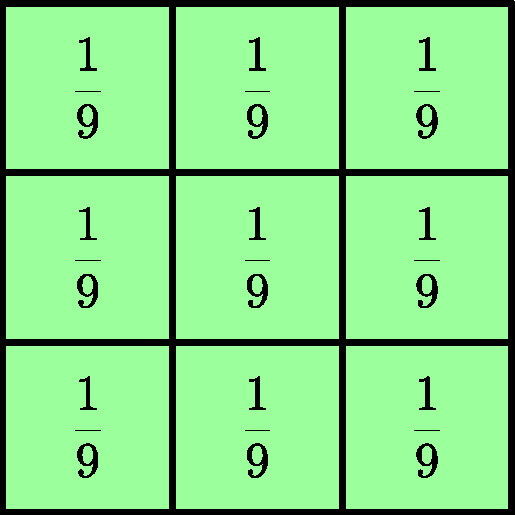
\includegraphics[height=2cm]{figs/maxmixed.pdf}
    %\caption{Maximally mixed state $\frac{1}{3}\id$}%
    }\hspace{8pt}%
    \subfigure[][]{%
    \label{fig:zero}%
    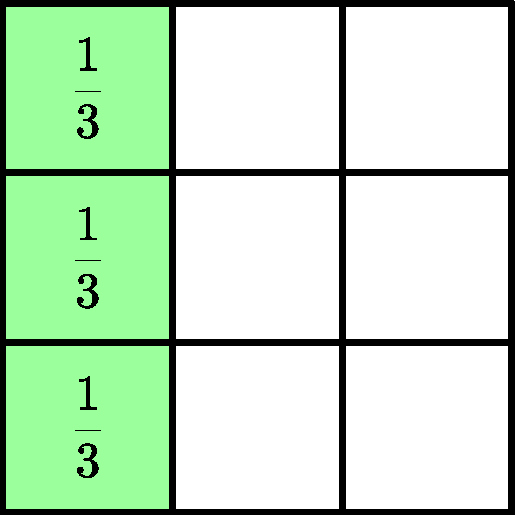
\includegraphics[height=2cm]{figs/zerostate.pdf}
    %\caption{Zero state $\ketbra{0}{0}$}%
    }\\
    \subfigure[][]{%
    \label{fig:bound}%
    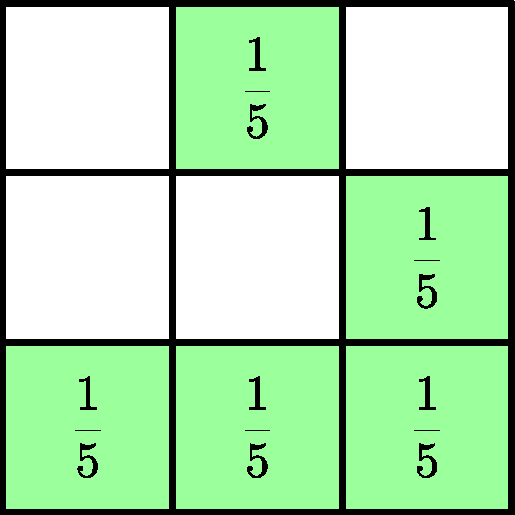
\includegraphics[height=2cm]{figs/boundstate.pdf}
    %\caption{Bound state}%
    }\hspace{8pt}%
    \subfigure[][]{%
    \label{fig:strange}%
    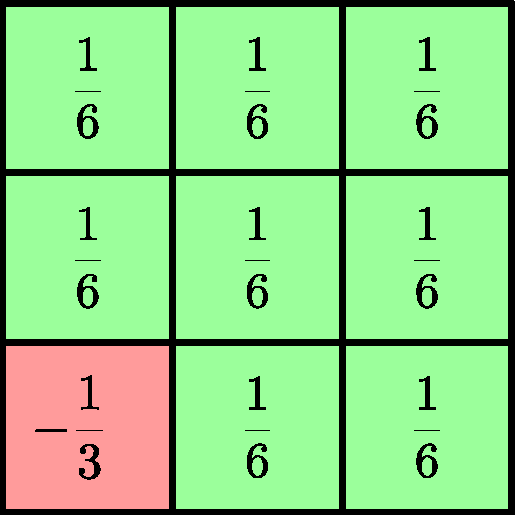
\includegraphics[height=2cm]{figs/strangestate.pdf}
    %\caption{Strange state $\ketbra{S}{S}$}%
    }
    \caption{\textbf{Qutrit Wigner distributions of varying magic.} 
    \subref{fig:maxmix} Maximally mixed state $\frac{1}{3}\id$; \subref{fig:zero} Stabilizer zero state $\ketbra{0}{0}$; \subref{fig:bound} A non-stabilizer Wigner-positive state; \subref{fig:strange} Magic strange state $\ket{{\rm{S}}} = \frac{1}{\sqrt{2}}(\ket{1} - \ket{2})$.
    \nick{Explain what a magic / bound magic state is in intro}
    }%
    \label{fig:wstate_examples}
\end{figure}

We can exploit the channel-state duality and use the normalised Choi-Jamio\l{}kowski state 
\begin{equation}\label{eq:cj}
    \frac{1}{d_A}\J(\E) \coloneqq \frac{1}{d_A}(\id \otimes \E) \sum_{i,j} \ket{ii}\bra{jj}
\end{equation}
to extend the definition of the Wigner distribution to quantum $\cptp$ operations $\E: \cal{B}(\hd[d_A]) \mapsto \cal{B}(\hd[d_B])$, 
\begin{align}\label{eq:woperation}
    \W[\bmy|\bmx]{\E} 
    &\coloneqq d_A^2 \W[\bm{\bar x} \oplus \bmy]{\frac{1}{d_A}\J(\E)} \\
    &= \frac{1}{d_B} \tr_B[A_{\bmy} \E(A_{\bmx})],
\end{align}
where $\bm{\bar x} \coloneqq (x_0, -x_1)$.

The specific form of~\cref{eq:woperation} is chosen so that Wigner distributions of operations act as transition matrices for Wigner distributions of states, $\W{\E(\rho)} = \W{\E}\W{\rho}$.
In particular, $\cptp$ operations that map between density operators of equal dimensions and have non-negative Wigner distributions correspond to stochastic matrices, as shown in~\cref{app:wigner}

The single-qudit Hadamard gate $H$ and phase gate $S$ generate the $d$-dimensional Clifford group $\cd$. \nick{CITE}
Their Wigner distributions are given by permutation matrices,
\begin{align}
    H &\coloneqq \frac{1}{\sqrt{d}}\sum_{j,k} \omega^{jk} \ketbra{j}{k}, \W[\bmy|\bmx]{H} = \delta_{y_0, -x_1}\delta_{y_1, x_0};\label{eq:H}\\
    S &\coloneqq \sum_k \tau^{k(k+1)} \ketbra{k}{k}, \W[\bmy|\bmx]{S} = \delta_{y_0, x_0}\delta_{y_1, x_0 + x_1 + 2^{-1}}.\label{eq:S}
\end{align}

%%%%%%%%%%%%%%%%%%%%%%%%%%%%%%%%%%%%%%%%

\section{Stochastic structure of magic theories}
\label{sec:struc}

\subsection{Magic fragments}\label{sec:magfrag}

Equipped with the definitions of the Wigner distribution in odd prime dimensions, we can formally recast the maximal magic theory $\Rmax$ into a stochasticity setting.
The free states correspond to proper probability distributions 
\begin{equation}
    \Fmax \coloneqq \{ \rho: \W[\bmz]{\rho} \geq 0 \text{ for all } \bmz \in \pd\}
\end{equation}

The free operations should send the set of free states $\Fmax$ into itself and completely preserve the non-negativity of the states, in the sense that $\E \in \Omax$ iff $(\id_d \otimes \E ) \sigma \in \stab$ for all odd prime dimensions $d$ whenever $\sigma \in \Fmax$.
It is shown by Wang \textit{et al.}~\cite{cit:wang} that $\Omax$ coincides with the set of operations $\E$ that correspond to stochastic Wigner distributions, 
\begin{equation}
    \Omax = \{ \E: \W[\bmy|\bmx]{\E} \geq 0 \text{ for all } \bmx, \bmy \in \pd\}.
\end{equation}

Any magic theory $\R = (\F, \O)$ is a subtheory of $\Rmax$ as explained in~\cref{sec:intro}, and as such it falls under this new stochasticity setting. 
For technical simplicity in what follows we assume that $\F$ is a closed set, and note that $\F_{\rm{ max}}$ is itself a closed set, since it is specified by a finite set of linear constraints of the form $\tr[ L\rho] \geq 0$ with operators $L \in \cal{B}(\cal{H})$ ensuring that the state is positive and Wigner-positive.


Given this context we now define the following key notion, that is central to our analysis.
\begin{definition}[\textbf{$\boldsymbol\sigma$-fragment}]\label{def:sigmafrag}
   Given a resource theory of magic $\R = (\F, \O)$, the \emph{$\sigma$--fragment of $\R$} is the resource theory $\R_\sigma = (\F, \O_\sigma)$, where the free operations are restricted to the ones that leave $\sigma$ invariant, namely
    \begin{equation}
        \O_\sigma \coloneqq \{ \E \in \O: \E(\sigma) = \sigma \}.
    \end{equation}
\end{definition}

With this basic notion defined, we now show that any resource theory of magic can be faithfully subdivided into $\sigma$--fragments, in such a way that any problem of interconversion in the parent magic theory $\R$ can be analysed across the different fragments.

\begin{theorem}
    Let $\R = (\F, \O)$ be a theory of magic.
    Every operation in $\O$ leaves at least one free state invariant,
  \begin{equation}
\O = \bigcup\limits_{\sigma \in \F} \O_\sigma.
\end{equation}
Therefore, $\rho \longrightarrow \tau$ in $\R$ if and only if $\rho \longrightarrow \tau$ in a $\sigma$--fragment of $\R$.
\end{theorem}
\begin{proof}
    Suppose $\E$ is in a $\sigma$--fragment $\O_\sigma$.
    Then it is also in $\O$, hence $\bigcup\limits_{\sigma \in \F} \O_\sigma \subseteq \O$. 
    
    Conversely, suppose $\E$ is in $\O$. 
    The free states are a closed set that is mapped one-to-one to a closed subset $\cal{S}$ of the $(d^2 - 1)$-dimensional probability simplex.
    $\cal{S}$ is convex, since any combination of free states is also free and the Wigner distribution is linear.
    Therefore, $\cal{S}$ is convex and compact as a closed convex subset of the bounded compact probability simplex.
    
    We can now view $\W{\E}$ as a stochastic, continuous mapping from $\cal{S}$ to itself, thus Brouwer's fixed point theorem \nick{CITE} implies that there exists a probability distribution $d_{\bmz}$ for some $ \bmz \in \pd$ that is a fixed point of $\W{\E}$.
    This corresponds to a free state $\sigma \coloneqq \sum_{\bmz \in \pd} d_{\bmz} A_{\bmz} \in \F$. 
    Therefore $\E \in \O_\sigma$, and so $\O = \bigcup\limits_{\sigma \in \F} \O_\sigma$. 
    
    The state interconversion result follows immediately.
\end{proof}

The zoo of all magic operation classes is summarised in ~\cref{fig:zoo}.
Completely positive-Wigner-preserving operations~\cite{cit:wang} form the operation class $\Omax$.
Therefore, $\sigma$--fragments cover this theory of magic exactly and any magic subtheory is contained within this cover.
In particular, the stabilizer operations $\so$ are contained within $\Omax$.
\begin{figure}[t]
    \centering
        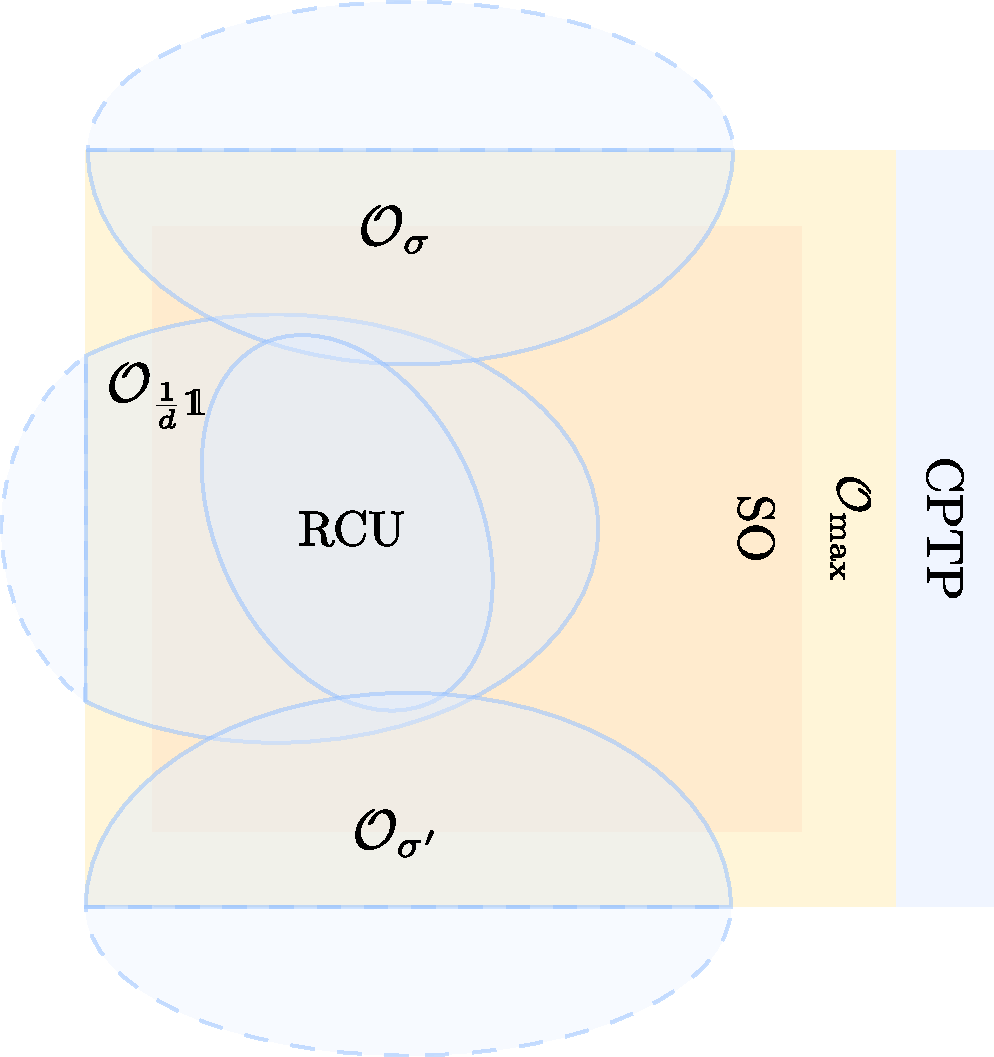
\includegraphics[scale=0.47
        ]{figs/operations.pdf}
    \caption{\textbf{Decomposition of a magic theory $\R$ intro $\sigma$--fragments.} 
    Examples of magic theories ($\so$: Stabilizer operations, $\Omax$: Completely positive-Wigner-preserving operations, $\rcu$: Random Clifford Unitaries -- subclass of $\so$) involve operations within the yellow regions, with all other established magic theories between these two.
    We introduce $\sigma$--fragments $\O_\sigma$ defined for all free states $\sigma$ that cover $\Omax$ with each one extendible to a set of stochastic maps outside the $\cptp$ operations.
    Within each $\sigma$--fragment $\bmd$-majorization can be used allowing for an \nick{in-depth approach} towards the study of magic state interconversion.
    }
    \label{fig:zoo}
\end{figure}

The subdivision of magic theories into $\sigma$--fragments is powerful because the pre-order $\prec_{\R_\sigma}$ of every $\sigma$--fragment is described by well-behaved majorization tools, as we establish in~\cref{sec:major}.

\subsection{Majorization of quasi-probabilities in the $\sigma$--fragments}\label{sec:major}

Majorization is a collection of powerful tools that has recently found many applications in quantum information theory \nick{CITE}.
It can describes the \nick{disorder / non-uniformity} of distributions that undergo stochastic transformations.

To formally state majorization results, we first denote by $\stoch$ the set of $(d \times d)$ stochastic matrices that preserve the probability vector $\bmd$. \nick{Should we introduce notation directly in the magic setting?}
Specifically, for any $S \in \stoch$, all matrix elements are non-negative, all rows sum to $1$ and $S\bmd = \bmd$.
\iffalse
\begin{enumerate}
    \item $S_{ij} \geq 0$ for all $i, j \in \zd$;
    \item $\sum\limits_{j=1}^n S_{ij} = 1$ for all $i \in \zd$;
    \item $S\bmd = \bmd$.
\end{enumerate}
\fi
The set $\stoch$ forms a group under matrix multiplication for all $\bmd$ with positive components.

Majorization finds an important application on quantum thermodynamics in the absence of coherence.
The use of majorization in this setting provides useful intuition for our purposes.
At any given temperature $\beta$, the thermal state $\gamma_\beta$ is thermodynamically the most disordered state. 
Thermal operations are defined as operations that cannot extract energy from the Gibbs state, $\E(\gamma_\beta) = \gamma_\beta$.
Convertibility between states via thermal operations is equivalent to a stochasticity condition on the energy level populations of the states \nick{CITE}.
Roughly, the statement is that there exists a thermal operation $\E$ such that $\tau = \E(\rho)$ if and only if there exists a a matrix $S \in \stoch$ such that $\bm{q} = S\bm{p}$, where $\bm{q}, \bm{p}$ and $\bmd$ and the energy level population vectors of $\tau, \rho, \gamma_\beta$ respectively.

Drawing intuition from this setting, we can define majorization as follows.
\begin{definition}[\textbf{$\boldsymbol\bmd$-majorization}]\label{def:dmajor}
    Given $\bmx, \bmy, \bmd \in \reals^d$, such that the components of $\bmd$ are positive, $\bmy$ is said to $\bmd$-majorize $\bmx$, iff there exists a matrix $S \in \stoch$ such that $\bmx = S\bmy$.
\end{definition}
We denote this pre-order by $\bmx \prec_{\bmd} \bmy$.
If $\bmd = \frac{1}{d}\bm{1}$, the $d$-dimensional uniform distribution, then $\stoch$ is the set of doubly stochastic matrices and we retrieve the familiar notion of majorization in entanglement theory. \nick{CITE}

The pre-order $\prec_{\R_\sigma}$ of the $\sigma$--fragment $\R_\sigma = (\F, \O_\sigma)$ between $d$-dimensional states corresponds to the majorization pre-order $\prec_{\W{\sigma}}$ between their $d^2$-dimensional Wigner distributions.
For simplicity we shall merge the notation into $\prec_\sigma$, as there is little risk of confusion.


\begin{theorem}\label{thm:sigmamajor}
    Let $\R = (\F, \O)$ be a theory of magic. Then $\rho \longrightarrow \tau$ is possible then  $\W{\tau} \prec_\sigma \W{\rho}$ within a $\sigma$--fragment.
\end{theorem}
\begin{proof}Suppose we can convert $\rho$ into $\tau$ in the magic theory. Thus there is some $\O_\sigma$ and some $\E \in \O_\sigma$ such that $\E(\rho) = \tau$, and $\E(\sigma)=\sigma$. Therefore, the Wigner distribution of this free operation satisfies $\W{\E} \in \stochw$ and $\W{\E}\W{\rho} = \W{\tau}$. Since $\sigma$ is full-rank and free, its Wigner distribution is strictly positive in all components, so it directly follows from~\cref{def:dmajor} that $\W{\tau} \prec_{\sigma} \W{\rho}$.
\end{proof}
This result can be understood as an extension of the idea of a magic monotone, where we replace $\M(\tau) \le \M(\rho)$ with $W_\tau \prec_\sigma W_\rho$. However the majorization constraints can be used to place upper bounds on magic state distillation in a way that allows one to incorporate the physics of the allowed operations -- this enables us to bound how much magic can be distilled via quantum operations that, for example, preserve the equilibrium state of the system, or via operations that are symmetric about the $Z$-axis of the Bloch sphere.

This approach can also provide \emph{lower bounds} on distillation, however now more structure about the specific free operations must be included. This is more involved and we discuss this later in the paper.

\subsection{Majorization computations in a $\sigma$--fragment}
A numerically efficient reformulation of $\bmd$-majorization is provided by Lorenz curves.
Let the vector $\bmu^\downarrow$ denote the vector $\bmu \in \reals^d$ with its components arranged in non-increasing order.
\begin{definition}[\textbf{Lorenz curve}]\label{def:lc}
    Let $\bmz, \bmd \in \reals^d$, where the components of $\bmd$ are positive with $D = \sum_{i=1}^d d_i$ and denote by $\bmu \coloneqq (z_1/d_1, \dots, z_d/d_d)^T$ the vector of ratios between the corresponding components of $\bmz$ and $\bmd$.
    
    Finally, denote by $\pi: \zd \mapsto \zd$ the permutation that sorts $\bmu$, $(\bmu^\downarrow)_i = u_{\pi(i)}$ for all $i=1,\dots,d$.
    
    Consider the piecewise linear curve obtained by joining the points $\{(0,0)\} \cup \{ (x_k, \lc{\bmz}{\bmd}(k)) \}_{k=1,\dots,d}$, where
    \begin{equation}\label{eq:lorenz}
        (x_k, \lc{\bmz}{\bmd}(k)) \coloneqq \left( \frac{1}{D}\sum_{i=1}^k d_{\pi(i)}, \sum_{i=1}^k z_{\pi(i)} \right) \in \mathbb{R}^2.
    \end{equation}
    The \emph{Lorenz curve} of vector $\bmz$ with respect to $\bmd$ is then $\lc{\bmz}{\bmd}(x)$ for all $x \in [0,1]$
    
    Expressed explicitly,
    \begin{equation}
		\lc{\rho}{\sigma}(x) = (\bmu^\downarrow)_i x + \lc{\rho}{\sigma}(i) - (\bmu^\downarrow)_i x_i,\ x \in (x_{i-1}, x_i],
	\end{equation}
	for all $i=1,\dots,d$ with $x_0 \coloneqq 0$.
\end{definition}
\nick{Move the complicated last equation to appendix?} \ddd{[Yes. Just describe in words, is simpler. the reader with being able to understand how to construct a piecewise linear function.]}
Components $x_k$ are rescaled by $D$ so that comparison of curves with unequal dimensions is possible.
In fact, the Lorenz curves $\lc{\bmz}{\bmd}$ and $\lc{\bmz \otimes \bmd}{\bmd \otimes \bmd}$, where $\otimes$ denotes the Kronecker product, are identical.
Furthermore, a Lorenz curve $\lc{\bmz}{\bmd}(x)$ is always concave in $x$, since it consists of $d$ line segments each with slope $(\bmu^\downarrow)_i$ for $i=1,\dots,d$ which is non-increasing by definition.

A vector $\bmy$ \emph{$\bmd$--majorizes} another vector $\bmx$ if and only if the Lorenz curve $\lc{\bmy}{\bmd}$ lies above Lorenz curve $\lc{\bmx}{\bmd}$, thus reducing $\bmd$--majorization into a finite set of inequalities.
\begin{theorem}\label{thm:dmajor}
    Let $\bmx, \bmy, \bmd \in \reals^d$, such that the components of $\bmd$ are positive. 
    Then, $\bmx \prec_{\bmd} \bmy$ if and only if $\lc{\bmx}{\bmd}(x) \leq \lc{\bmy}{\bmd}(x)$ for all $x \in [0,1]$ with strict equality at $x=1$.
\end{theorem}
A restatement of the theorem including more equivalent conditions and a proof are provided in~\cref{app:major}.
An example of comparison between different Lorenz curves is illustrated in~\cref{fig:lctoy}.\nick{move around}
\begin{figure}
    \centering
    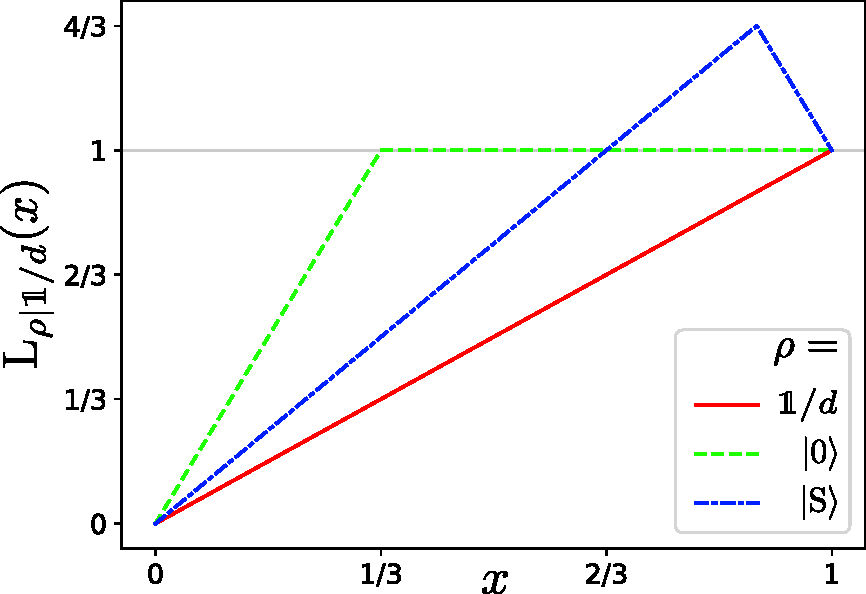
\includegraphics[height=5cm]{figs/lctoy.pdf}
    \caption{Example of different Lorenz curves for quasi-probability vectors under $\bmd$-majorization.
    Vectors $\bmy$ and $\bmd$ are simply probability distributions.
    The curve corresponding to vector $\bmd$ is always the line segment connecting $(0,0)$ and $(1,1)$, so that any other Lorenz curve lies above it, for example $\bmx \prec_{\bmd} \bmd$.
    Curves $L_k(\bmx|\bmd)$ and $L_k(\bmy|\bmd)$ intersect, so $\bmx \nprec_{\bmd} \bmy$ as well as $\bmy \nprec_{\bmd} \bmx$.
    \nick{Recast in terms of magic - replace with~\cref{fig:test}?}
    }
    \label{fig:lctoy}
\end{figure}

It is now straightforward to construct Lorenz curves for Wigner distributions in any $\sigma$--fragment.
As we have seen in~\cref{thm:sigmamajor}, for any full-rank free state $\sigma$ we have that $\W{\sigma}$ is a strictly positive full-rank probability distribution, and so one can define a corresponding notion of $d$--majorization on \emph{quasi}--distributions.
We write $\lc{\rho}{\sigma}(x)$ for the Lorenz curve of $\W{\rho}$ with respect to $\W{\sigma}$.

We now establish important properties of Lorenz curves that are independent of the $\sigma$--fragment they are defined in.
\begin{proposition}\label{thm:lccont}
	The Lorenz curve $\lc{\rho}{\sigma}(x)$ of a state $\rho$ with respect to state $\sigma$ is uniformly continuous in $\sigma$. 
	\nick{In the sense that if $\sigma$ and $\sigma'$ are $\delta$-close with respect to a state norm, then the curves $\lc{\rho}{\sigma}(x)$ and $\lc{\rho}{\sigma'}(x)$ are $\epsilon$-close at all $x \in [0,1]$.
	I think this clears up the narrative quite a bit? - Should we keep and prove this result?} \ddd{[Is a nice result...hmm let's wait and see. It might distract from the main message.]}
\end{proposition}
The proof of this important result is in \nick{the appendix}.
The consequence of this statement is that infinitesimal changes in state $\sigma$ only result in infinitesimal shifts of the $\sigma$--fragment.
Therefore, Lorenz curves and majorization analysis in general \nick{behave nicely in the presence of / are robust under} imperfections in the experimental implementation of quantum operations.
In particular, any $\sigma_0$--fragment defined by a non full-rank state $\sigma_0$ can be approximated by a $\sigma$--fragment defined by a full-rank $\sigma$ which is arbitrarily close to $\sigma_0$, such that $\sigma = (1-\epsilon)\sigma_0 + \epsilon\frac{1}{d}\id$, for some small $\epsilon > 0$.
Such $\sigma_0$--fragments may include important stabilizer operations such that the replacement channel defined as $\E(\rho) = \sigma_0$ for all states $\rho$.
For simplicity, we restrict analysis to $\sigma$-fragments, where $\sigma$ is full-rank.

Normalisation of the Wigner distribution \nick{REF} ensures that for all quantum states $\rho$, $\lc{\rho}{\sigma}(x) \geq 0$ and $\lc{\rho}{\sigma}(1) = 1$.
As a consequence, checking whether a state conversion $\rho \longrightarrow \tau$ is possible as per~\cref{thm:dmajor}, reduces to the condition $\lc{\rho}{\sigma}(x) \leq \lc{\tau}{\sigma}(x)$ for all $x \in [0,1]$.
We stress that $0 \leq \lc{\rho}{\sigma}(x) \leq 1$ for all $x \in [0,1]$ if and only if $\rho$ is a positive Wigner state.

The area $\A_\sigma(\rho)$ between the curve $L_{\rho|\sigma}$ and the line $y=1$ is a resource monotone in the $\sigma$--fragment. 
This is clear because for any state conversion $\rho \longrightarrow \tau$ for some $\E \in \O_\sigma$, the Lorenz curve $L_{\tau|\sigma}$ is lower than $L_{\rho|\sigma}$, hence $\A_\sigma(\E(\rho)) \leq \A_\sigma(\rho)$.
The exact form of the monotone is given in~\cref{app:areamono}

\ddd{[relate to mana?]} \nick{the area depends on several positive Wigner components and cannot be written as a function of mana annoyingly - should we include the area? Have a look at~\cref{app:areamono}}


%%%%%%%%%%%%%%%%%%%%%%%%%%%%%%%%%%%%%%%%


%%%%%%%%%%%%%%%%%%%%%%%%%%%%%%%%%%%%%%%%%

\section{Magic state interconversion and Lorenz curves}
\label{sec:distill}

Any quantum circuit aiming at a given magic state conversion $\rho \longrightarrow \tau$ possesses certain symmetries according to~\cref{thm:frag} that allow us to study the conversion within only certain $\sigma$-fragments.
As a simple example, the dephasing channel
\begin{equation}\label{eq:dephase}
	\Delta(\rho) = \sum_{k \in \zd} \ketbra{k}{k}\rho\ketbra{k}{k}
\end{equation}
removes coherent phases in the computational basis and therefore leaves exactly all mixtures of computational basis states invariant.
A model circuit consisting only of such dephasing channels can be fully analysed in the $\sigma$--fragments for the pure computational basis states $\sigma$ \nick{as seen in a theorem in the appendix}.

Lorenz curves provide an efficient method of numerically checking if a certain state conversion is impossible within a $\sigma$--fragment by exploiting the equivalence with $d$--majorization stated in~\cref{thm:dmajor}.
Such methods are often more conclusive than magic monotones as we discuss in section~\cref{sec:scmana}.

\subsection{Mana and majorization in magic theories}\label{sec:scmana}
We now discuss majorization features common to all fragments, before specialising to particular $\sigma$--fragments and how analysis in them proceeds. 
Mana is the fundamental resource monotone for magic. 
Here we show that its properties are in fact special cases of more general majorization features. 
More precisely, its properties can be viewed as majorization-based, and independent of the particular $\sigma$--fragment one works in.

As discussed above, we know that every magic interconversion problem can be analysed across all $\sigma$--fragments that reflect symmetries of the circuit and moreover the pre-order in each such fragment is exactly specified by $d$--majorization.

Consider a general magic state interconversion in $\O_\sigma$, $\rho \xrightarrow{\E \in \O_\sigma} \tau$.
It is shown in~\cref{app:major} that mana is an additive monotone in every $\sigma$--fragment under $d$--majorization, so it provides a necessary condition for the process to be possible,
\begin{equation}\label{eq:manabound}
    \mana{\rho} \geq \mana{\tau}. %{\rm{C}}_{\rm{mana}}(\rho, \tau, \sigma):\ 
\end{equation}
A new bound can be obtained in the $\sigma$--fragment by comparing the Lorenz curves of the initial and target states,
\begin{equation}\label{eq:majbound}
    \lc{\rho}{\sigma}(x) \geq \lc{\tau}{\sigma}(x),\ x\in [0,1].
\end{equation}
If one of these consitions is not satisfied, then the Lorenz curve of initial state $\rho$ is below the curve of target $\tau$ at some point $x$ and the conversion is not possible.

In fact, our current setting makes it apparent that the mana condition is always weaker than the majorization condition for all magic state interconversions.

We first show that the maximum of $\lc{\rho}{\sigma}$ is independent of the $\sigma$--fragment and directly related to the state sum-negativity $\sn{\rho}$ discussed in~\cref{sec:mono}
\begin{lemma}\label{lem:lcmax}
	Given a quantum state $\rho$, the maximum of its Lorenz curve $\lc{\rho}{\sigma}$ is independent of the $\sigma$--fragment in which it is defined and equal to $1+\sn{\rho}$.
\end{lemma}
\begin{proof}
	Borrowing the notation of~\cref{def:lc}, the derivative of the Lorenz curve $\lc{\rho}{\sigma}$ is
	\begin{equation}
		\frac{\rm{d}}{\rm{d}x} \lc{\rho}{\sigma}(x) = (\bmu^\downarrow)_i,\ x \in (x_{i-1}, x_i],
	\end{equation}
\ddd{[The function is not differentiable at the key points involved. The maximum is obtained when you sum all the non-negative components.]}

	Note that all components of $\W{\sigma}$ are positive, so $(\bmu^\downarrow)_i \geq 0$ if and only if $(\W{\rho})_i \geq 0$ for any $i=1,\dots,d^2$.

	Suppose all components of $\W{\rho}$ are non-negative.
	Then, $\sn{\rho}=0$ and the global maximum of the Lorenz curve is dictated by the normalisation of $\W{\rho}$ so we trivially have
	\begin{equation}
		\max_{x\in[0,1]}{\lc{\rho}{\sigma}(x)} = 1 = 1 + \sn{\rho}.
	\end{equation}
	
	Suppose that $\W{\rho}$ has at least one negative component.
	Let $k$ be the index of the smallest non-negative component of $\bmu^\downarrow$.
	Then the maximum of the Lorenz curve $\lc{\rho}{\sigma}$ occurs at $x_k$, just before its slope becomes negative. 
	The $x$-coordinate $x_k$ is different for different $\sigma$--fragments but the value of the maximum is the same and is given by
	\begin{align}
		&\max_{x\in[0,1]}{\lc{\rho}{\sigma}(x)}
		= \lc{\rho}{\sigma}(x_k)
		= \sum\limits_{i=1}^k (\W{\rho})_{\pi(i)} \\
		&= \sum\limits_{\bmx: \W[\bmx]{\rho} \geq 0} \W[\bmx]{\rho}
		= 1 + \sn{\rho}.
	\end{align}
	
\end{proof}
\nick{Perhaps create Lorenz curve appendix and put the proof there as well as how functional form and discretised form of Lorenz curves relate}
\ddd{[This I think is a simpler approach:]}
The Lorenz curve of $L_{\bmx |\bmd}(x)$ is defined by piecewise linear sections sequentially linking the points $\{ (a_k,b_k)\}$ where $a_k = \sum_{i=1}^k x_i$, $ b_k = \sum_{i=1}^k d_i$ and we order the components such that $\tilde{x}_i:=x_i / d_i$ form a non-increasing sequence in $i$.

Now let $k_\star$ be the index of the smallest non-negative number in $(\tilde{x}_i)$, and define 
\begin{align}
a_\star &:= \sum_{i=1}^{k_\star} x_i\\
b_\star &:= \sum_{i=1}^{k_\star} d_i.
\end{align}
It is then clear that $L_{\rho|\sigma}(x)$ attains a maximum value of $a_\star \ge 1$ at the point $x = d_\star$.

Note that since $\bmd \ge \mathbf{0}$, for $i > k_\star$ we have that $x_i \le 0$, independent of the particular $\bmd$ we use. Therefore the value of $a_\star$ is independent of the particular fragment, with only the location of the maximum ($x=b_\star$) varying from fragment to fragment. \ddd{[This method is tidier.]}

We can therefore view mana as one of the features of the Lorenz curve, its maximum.
\begin{theorem}\label{thm:bounds}
    Given a magic state conversion $\rho \longrightarrow \tau$, the majorization condition is stronger than the mana condition in all $\sigma$--fragments.
\end{theorem}
\begin{proof}
    The maximum of the Lorenz curve of a state $\rho$ is independent of the $\sigma$--fragment due to~\cref{lem:lcmax}, and can be expressed as an increasing function of mana,
    \begin{equation}
        \max_{x\in[0,1]}{\lc{\rho}{\sigma}(x)} = 1 + \sn{\rho} = \frac{1}{2} \left( 1 + e^\mana{\rho} \right).
    \end{equation}
    Therefore, the $\W{\sigma}$--majorization bound
    \begin{equation}
    	\lc{\rho}{\sigma}(x) \geq \lc{\rho}{\sigma}(x),\ x\in[0,1]
    \end{equation}
    implies the order $\max_{x\in[0,1]}{\lc{\rho}{\sigma}(x)} \geq \max_{x\in[0,1]}{\lc{\rho}{\sigma}(x)}$ which is equivalent to the mana bound $\mana{\rho} \geq \mana{\tau}$.
\end{proof}

Of practical importance are magic state distillation (MSD) processes of the form
\begin{equation}\label{eq:distprocess}
    \rho^{\otimes k} \xrightarrow{\E \in \O_\sigma} \tau,
\end{equation}
where $k$ copies of a noisy magic state $\rho$ are converted into a target single-copy state $\tau$. \nick{expand?}

In general, the Wigner components of a $k$-copy state $\rho^{\otimes k}$ can be calculated, along with their multiplicities, from $W_\rho$ by expanding the terms in the multinomial expansion $\left( \sum_{\bm{z} \in \cal{P}_d} W_\rho(\bm{z}) \right)^n$.
This follows from the multiplicativity of the Wigner distribution.

As an example, consider a qutrit distillation process involving the Strange state $\ketbra{\rm{S}}$ depicted in~\cref{fig:strange}. 
It is the simplest non-trivial case to analyse, since the Strange state only has two distinct components $\left\{ -\frac{1}{3}, \frac{1}{6} \right\}$ with multiplicities $1$ and $8$ respectively.
Calculating the binomial expansion for the components of $\ket{S}\bra{S}^{\otimes k}$ gives $\{(-1)^j 2^{j-k} 3^{-k}\}_{0 \leq j \leq k}$ with multiplicity $8^{k-j} \binom{k}{j}$ for the $j$-th term.
This allows analytical calculation of all Lorenz curve points, and for the $k$-copy state we have that
\begin{equation}\label{eq:Skmax}
    \max_x{\lc{\ketbra{S}^{\otimes k}} {\sigma}}(x) = \frac{1}{2}\left (1 + \left(\frac{5}{3}\right)^k \right),
\end{equation}
independent of the particular $\sigma$--fragment. \ddd{[We should also give for what value of $x$ this maximum occurs.]} 
%1 + \left(\frac{4}{3}\right)^k \sum\limits_{j=0}^{\floor{\frac{k-1}{2}}} 4^{-(2j+1)} \binom{k}{2j+1}
%\sum_{n=1, n \mbox{ odd}}^k a^n \binom{k}{n} = \frac{1}{2} \left [  (1+a)^k - (1-a)^k \right ]

\subsection{Distilling out magic in a fragment}
Consider, as an example, the problem of purifying out magic from a noisy state of the form
\begin{equation}
    \rho_{\rm{S}}(\epsilon) = (1 - \epsilon) \ket{\rm{S}}\bra{\rm{S}} + \epsilon \sigma,
\end{equation}
in $\O_\sigma$.
At noise levels $\epsilon \geq \frac{3}{4}$, the state is sufficiently noisy so as the Wigner distribution $\W{\rho_{\rm{S}}(\epsilon)}$ no longer contains negativities. 
At any $\epsilon \leq \frac{3}{4}$, we can investigate the distillation process resulting in a single-copy state with sufficiently low target $\epsilon_{\tau}$,
\begin{equation}\label{eq:sdist}
	\rho_{\rm{S}}(\epsilon)^{\otimes k} \xrightarrow{\E \in \O_\sigma} \rho_{\rm{S}}(\epsilon_{\tau})
\end{equation}

The more noisy the initial state is, the more copies needed to reach the target, therefore it makes sense to define a noise level threshold
\begin{equation}\label{eq:ethresh}
	\epsilon_{\rm{th}}(k, \epsilon_\tau, \sigma) \coloneqq \sup{\{\epsilon:\ \lc{\rho_{\rm{S}}(\epsilon)^{\otimes k}}{\sigma} \geq \lc{\rho_{\rm{S}}(\epsilon_{\tau})}{\sigma}\}},
\end{equation}
so that the MSD process~(\ref{eq:sdist}) is impossible for all $\epsilon > \epsilon_{\rm{th}}(k, \epsilon_\tau, \sigma)$

\nick{Condition in~\cref{eq:ethresh} is informally written. Can also define 
\begin{equation}\label{eq:ethresh}
	k_{\rm{th}}(\epsilon, \epsilon_\tau, \sigma) \coloneqq \min{\{k:\ k \in \mathbb{N}, \lc{\rho_{\rm{S}}(\epsilon)^{\otimes k}}{\sigma} \geq \lc{\rho_{\rm{S}}(\epsilon_{\tau})}{\sigma}\}}.
\end{equation}}
We now examine the MSD process~(\ref{eq:sdist}) in greater detail for some important $\sigma$--fragments.

\subsection{Magic in unital fragments}\label{sec:unital}

Magic state distillation circuits in principle consist of bulk sequences of random Clifford unitaries ($\rcu$)\nick{CITE}, depicted in~\cref{fig:zoo}.
Operations in $\rcu$ can be expressed as
\begin{equation}
    \E(\rho) = \sum_i p_i U_i \rho U_i^\dagger,\ U_i \in \cd.
\end{equation}
Depending on the symmetries of such operations, a sequence of them may belong in various $\sigma$--fragments and the majorization condition~(\ref{eq:majbound}) needs to be checked in all these $\sigma$-fragments that reflect the symmetries of the operation sequence.
However, they always belong to the \emph{unital fragment} $\O_{\frac{1}{d}\id}$

If one incorporates noisy channels in the circuit, for example dephasing channels as in~\cref{eq:dephase} in various bases, symmetries are reduced.
Dephasing channels and general bit-flip error channels are examples of the many error-inducing channels that respect the unital symmetry. \nick{expand}

\nick{Replace the following with discussion of MSD process in the unital fragment for various numbers of copies $k$ vs mana}

In~\cref{fig:distill}, we examine the purifying process 
\begin{equation}\label{eq:purify}
    \rho_{\rm{S}}^{\otimes k}(\epsilon_{\rm{th}}) \xrightarrow{\E \in \O_\sigma} \rho_{\rm{S}}(0.05),\ \sigma = (1-p)\ketbra{0} + p \frac{1}{3}\id
\end{equation}
with $\epsilon_{\rm{th}}$ being the noise level threshold that does not prohibit the process for given number of copies $k$ and $\sigma$--fragment, parametrised by $p$ as a mixture of the zero and the maximally mixed states.
Thresholds provided by Lorenz curve comparison are always much stricter than mana thresholds.
\begin{figure}
    \centering
    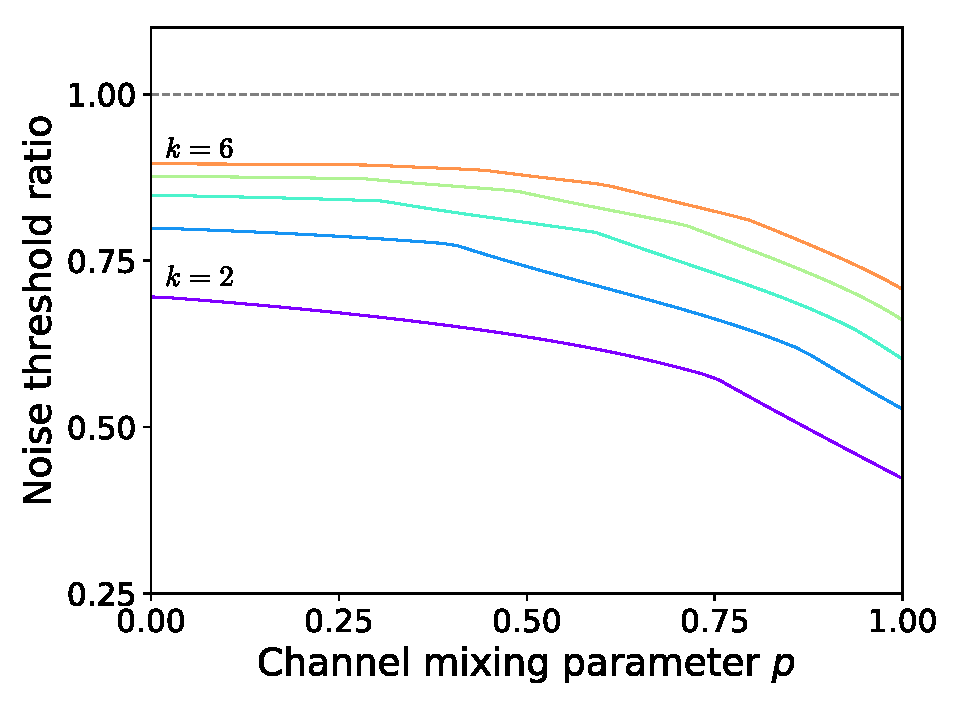
\includegraphics[scale=0.5]{figs/ratios.pdf}
    \caption{\textbf{Noise threshold ratios.} Mana and Lorenz curve ratios for the Strange state purifying process in~\cref{eq:purify}.
    The ratios are calculated for different numbers of initial state copies and different $\sigma$--fragments parametrised by $p$ such that $\sigma = (1-p)\ketbra{0} + p \frac{1}{3}\id$.
    Lorenz curve comparison consistently gives stricter bounds as proven in~\cref{thm:bounds}.
    \nick{Consider set of pure stabilizer states instead of $(1-p)\ketbra{0} + p \frac{1}{3}\id$ perhaps}
    }
    \label{fig:distill}
\end{figure}

\subsection{Magic in thermal fragments}\label{sec:thermal}

Consider a system driven by Hamiltonian $H$ and a circuit consisting of thermal operations.
The computational basis now coincides with the energy eigenbasis of Hamiltonian $H$.
We denote the thermal state $\gamma_\beta = \frac{e^{-\beta H}}{\Z_\beta}$, where $\Z_\beta = \tr[e^{-\beta H}]$.\nick{expand}

Thermal operations coincide with fragment $\O_{\gamma_\beta}$ \nick{expand}
The Wigner distribution of thermal state $\gamma_\beta$ always consists of strictly positive components,
\begin{equation}
	\W[\bmx]{\gamma_\beta} = \frac{e^{-\beta \epsilon_{x_0}}}{d\Z_\beta}\ \text{for all}\ \bmx \in \pd,
\end{equation}
so pre-order $\prec_{\gamma_\beta}$ is well defined.

We generalise the analysis of~\cref{sec:unital} \nick{expand}.
\nick{Include figure with noise threshold level $\epsilon_{\rm{th}}$ in $y$-axis and temperature $\beta$ in $x$-axis. for various numbers of copies $k$.}

\section{Extension to general quantum resource theories}
\label{sec:frag}

In the previous section we introduced the notion of $\sigma$--fragments for any resource theory of magic. In this section we pause to generalise this concept to an arbitrary resource theory and explain precisely how it connects with resource monotones. The busy reader more focussed on magic may skip this section.

State convertibility within a given resource theory is often a hard question to address due to the intricate structure of the theory.
In general, the structure of a theory $\R$ is described by a pre-order $\prec_\R$ and usually resource monotones are employed to reduce this structure into a simple real number ordering\nick{CITE}.
The subdivisions of magic theories into $\sigma$--fragments suggests a new approach towards investigating state convertibility which retains more structure of the origin theory than a measure can.

\subsection{Monotones}\label{sec:mono}

We highlight the defining property of a monotone for the discussion that follows.
\begin{definition}[\textbf{Resource monotone}]\label{def:mono}
    Let $\R = (\F, \O)$ be a resource theory.
    A resource monotone $\M$ is a projection from the set of quantum states of the theory onto the real line, so that $\M$ is monotonically decreasing under free operations,
    \begin{equation}
        \M(\rho_1) \leq \M(\rho_2)\ \text{whenever}\ \rho_1 \prec_{\R} \rho_2.
    \end{equation}
\end{definition}
The monotonicity condition reflects the no resource generating property of free operations, so that monotones respect the pre-order $\prec_\R$ of the theory.
Furthermore, a monotone may also satisfy the additivity condition,
\begin{equation}
    \M(\rho_1 \otimes \rho_2) = \M(\rho_1) + \M(\rho_2).
\end{equation}
This optional condition is of practical importance for resource distillation, which we discuss in~\cref{sec:distill} within the context of magic.

The most fundamental and commonly used magic monotone is the \emph{mana} of a state \nick{CITE}, defined as
\begin{equation}
    \mana{\rho} \coloneqq \log{\left(\sum\limits_{\bmz \in \pd} \abs{\W[\bmz]{\rho}}\right)}.
\end{equation}
It is a monotone function of the $\ell_1$-norm of the Wigner distribution that satisfies the additivity condition.
In particular, mana can be re-expressed as $\mana{\rho} = \log{(2\sn{\rho}+1)}$, where the sum-negativity ($\rm{sn}$) \nick{CITE} is the sum of the negative components in $\W{\rho}$,
\begin{equation}
	\sn{\rho} = \sum\limits_{\bmx: \W[\bmx]{\rho} < 0} \abs{\W[\bmx]{\rho}}.
\end{equation}

\subsection{Fragments}

Monotones reduce the structure of the resource theory $\R$ to a \emph{total} order on the real numbers.
Therefore, two states, even if incomparable in $\R$, are always mapped onto ordered real numbers.
We now generalise this idea of a theory projection that preserves comparability between states. 
\begin{definition}[\textbf{Covariant projection}]\label{def:covproj}
Let $\R = (\F, \O)$ be a resource theory with pre-order $\prec_\R$. 
Then a \emph{covariant resource projection} of $\R$ to a resource theory $\R'$ with pre-order $\prec_{\R'}$, is a pair of mappings $(\Pi_s, \Pi_o)$, where $\Pi_s$ maps quantum states in $\R$ to quantum states in $\R'$, and $\Pi_o$ maps free operations in $\R$ to free operations in $\R'$. 
Moreover, these obey
	\begin{enumerate}
        \item $\Pis(\rho_1) \prec_{\R'} \Pis(\rho_2)$ whenever $\rho_1 \prec_\R \rho_2$;
        \item $\Pio(\E) = \Pio(\E_1) \circ \Pio(\E_2)$ whenever $\E = \E_1 \circ \E_2$.
    \end{enumerate}
We call $\R'$ a \emph{covariant fragment} of $\R$.
\end{definition}

Resource monotones can now be clearly seen as a special case of covariant resource projections.
\begin{proposition}[\textbf{Totally ordered covariant theories}]\label{thm:monoproj}
	Any resource monotone $\M$ of a resource theory $\R$ is a covariant projection for which $\prec_{\R'}$ is a total order. 
	Conversely, any such covariant projection corresponds to a resource monotone $\M$. 
\end{proposition}
\begin{proof}
	Consider a monotone $\M$ in the context of a general resource theory $\R = (\F, \O)$.
	State order is covariantly preserved due to the defining property of a monotone, stated in~\cref{def:mono}, where the pre-order $\prec_{\R'}$ is simply the total order $\leq$ on $\mathbb{R}$. 
	
	Operational composition is covariantly preserved when we simply choose $\Pio(\E) = 1_\times$, namely the `multiplication by 1' operation on real numbers. 
	The definition of a resource monotone then automatically implies covariance.
	
	Conversely, given any covariant projection of $\R$ for which $\prec_{\R'}$ is a total order, we may map the totally ordered set of elements $\Pis(\rho)$ via an injective, non-decreasing function $f$ into $\mathbb{R}$. 
	Then, $\M(\rho):=f(\Pi_s(\rho))$ provides a numerical value for each $\rho$ that obeys the definition of a monotone.
	
\end{proof}

We can also view $\sigma$--fragments as an example of reducing the structure of a magic theory $\R$ to a subtheory with a tractable pre-order.
However, states which are incomparable in $\R$ remain incomparable and conversions between states which are comparable in $\R$ may no longer be possible.
\begin{definition}[\textbf{Contravariant projection}]\label{def:contraproj}
	Let $\R = (\F, \O)$ be a resource theory with pre-order $\prec_\R$. 
Then a \emph{contravariant resource projection} of $\R$ onto a resource theory $\R'$ with pre-order $\prec_{\R'}$, is a pair of mappings $(\Pi_s, \Pi_o)$, where $\Pi_s$ maps quantum states in $\R$ onto quantum states in $\R'$, and $\Pi_o$ maps free operations in $\R$ onto free operations in $\R'$. 
Moreover, these obey
	\begin{enumerate}
        \item $\rho_1 \prec_\R \rho_2$ whenever $\Pis(\rho_1) \prec_{\R'} \Pis(\rho_2)$;
        \item $\E = \E_1 \circ \E_2$ whenever $\Pio(\E) = \Pio(\E_1) \circ \Pio(\E_2)$.
    \end{enumerate}
We call $\R'$ a \emph{contravariant fragment} of $\R$.
\end{definition}
Note that a contravariant projection is always a surjective mapping for both states and operations, so that the conditions in~\cref{def:contraproj} make sense.
The use of covariant and contravariant in~\cref{def:covproj,def:contraproj} refers to the direction of implication between the two pre-orders and operation compositions\footnote{Note that strictly these are not projections in the sense of $\Pi^2 = \Pi$, but are instead morphisms. 
Here our use of the term projection is motivated by the idea that one one generally loses information about $\R$ under the mapping.}.

\begin{proposition}\label{thm:subproj}
    Let $\R = (\F, \O)$ be a resource theory, and let $\O' \subseteq \O$ be a non-empty subset of the free operations that is closed under composition, and moreover $\O'$ is the largest such subset, in the sense that for any $\E_1 \not \in \O'$ and any $\E_2 \in \O'$ we have that both $\E_1 \circ \E_2$ and $\E_2 \circ \E_1$ are not in $\O'$. Then $\R' = (\F, \O')$ of $\R$ defines a contravariant fragment of $\R$.    
\end{proposition}
\begin{proof}
    We first define $\Pis (\rho) = \rho$ for all $\rho$. It is clear that since $\O'$ is a subset of $\O$ any operation in $\O'$ will map the set of free states into itself. Moreover the identity channel $id$ is necessarily in $\O'$, due to the maximality assumption. For $\Pio$ we let $\Pis(\E) = \E$ if $\E \in \O'$ and otherwise $\Pis(\E) =id$. Now consider $\Pio (\E_1 \circ \E_2)$. Either the triple $\{\E_1, \E_2, \E_1\circ \E_2\}$ are all in $\O'$ or they are all outside of $\O'$. For the former case $\Pio(\E_1 \circ \E_2) = \E_1 \circ \E_2 = \Pio(\E_1) \circ \Pio(\E_2)$, while for the latter $\Pio(\E_1 \circ \E_2) = id = \Pio(\E_1) \circ \Pio(\E_2)$, which proves that compositions are respected under the map. Finally, $\rho \prec_{R'} \sigma$ implies there exists $\E \in \O' \subseteq \O$ such that $ \E(\rho) = \sigma$, and since $\E \in \O$ this implies $\rho \prec _{\R} \sigma$, as required, which completes the proof.
    
\end{proof}
\nick{Suppose $\E_2$ is the replacement channel $\E_2(\rho) = \sigma$. This is a stabilizer operation. Then $\E_2 \circ \E_1 \in \O_\sigma$ even if $\E_1 \notin \O_\sigma$. Now suppose $\E$ is a Hadamard unitary, then $id = \E \circ \E_{reverse}$ but $id \in \O_{\ketbra{0}}$ while $\E, \E_{reverse} \notin \O_{\ketbra{0}}$.} \ddd{[Ah ok, agreed. This is fine for now. Let's not spend ages trying to generalise this so as to include the majorization fragments. It's just good to explore the possibilities a bit, to illustrate the non-trivial aspects.]}
As an immediate corollary of~\cref{thm:subproj}, a $\sigma$--fragment of any magic theory $\R$ is a contravariant fragment of $\R$.


\begin{proposition}
	Let $\R = (\F,\O)$ be a resource theory, and let $\D \in \O$ be a free operation, which is reversible by $\D_{\rm{rev}} \in \O$, so that $\D_{\rm{rev}} \circ \D = \idc$.
	
	Then, we can define a contravariant projection of $\R$, by acting on all quantum states with $\D$.
\end{proposition}
\begin{proof}
	We show that the theory $\R' = (\F', \O)$, with $\F' = \{\D(\rho):\rho \in \F \}$, is a contravariant fragment of $\R$.
	
	Let $\Pis$ map every state $\rho$ to $\D(\rho)$ and suppose $\D(\rho_1) \prec \D(\rho_2)$. 
	Then, there exists $\E \in \O$ such that $\rho_1 = (\D_{\rm{rev}} \circ \E \circ \D) (\rho_2)$, so $\rho_1 \prec \rho_2$.
	
	Finally, let $\Pio$ map every free operation to itself, so that composition of operations is trivially preserved.
	
\nick{If $\D$ is a recovery map, so that $\D \circ \D_{\rm{rev}} = \idc$, then this is a covariant projection instead.

If $\D$ is not reversible, this mapping is in general NOT contravariant (consider the replacement map $\D(\rho) = \frac{1}{d}\id$ for a strange state and stabilizer state - surely there is such a counterexample in thermodynamics theory if we consider a highly coherent state and one with the same energy population but no coherences.} \ddd{[Ok. Again, let's not spend time worrying about this now. It's clear there is various fine-print to these cases...but they're not essential to our work so let's put this on hold.]}
\end{proof}

Important examples of resource fragments appear in several established resource theories. \nick{Need to check if the thermodynamics example works, include magic theories as fragments of $\Rmax$, include Nielsen's bipartite entanglement.} \ddd{[Don't worry about these things now -- let's get the computations section improved]}

\newpage

%%%%%%%%%%%%%%%%%%%%%%%%%%%%%%%%%%%%%%%%

\section{Conclusion}
\label{sec:conc}

\begin{enumerate}
    \item Introduced fragments
    \item Identify symmetries of the setup
    \item Combined single-shot thermodynamics with magic 
    \item Can we solve other cases exactly? (apart from single qutrit)
\end{enumerate}

%%%%%%%%%%%%%%%%%%%%%%%%%%%%%%%%%%%%%%%%

\bibliography{bib}
%\bibliographystyle{apsrev4-2}

%%%%%%%%%%%%%%%%%%%%%%%%%%%%%%%%%%%%%%%%

\appendix
\section{Properties of majorization}
\label{app:major}

\subsection{Equivalent conditions for majorization}

\begin{theorem}
Given $\bmx, \bmy, \bmd \in \mathbb{R}^n$, such that the components of $\bmd$ are positive, the following statements are equivalent:
 \begin{enumerate}
	\item[(TM1)] $\bmx \prec_{\bmd} \bmy$;
	\item[(TM2)] $\Gamma_{\bmd}({\bmx}) \prec \Gamma_{\bmd}({\bmy})$;
	\item[(TM3)]\label{en:tm3} $\sum\limits_{i=1}^n \abs{x_i - t d_i} \leq \sum\limits_{i=1}^n \abs{y_i - t d_i}$ for all $t \in \mathbb{R}$;
	\item[(TM4)] $\sum\limits_{i=1}^n (x_i - t d_i)^+ \leq \sum\limits_{i=1}^n (y_i - t d_i)^+$ for all $t \in \mathbb{R}$ and $\sum\limits_{i=1}^n x_i = \sum\limits_{i=1}^n y_i$;
	\item[(TM5)] $\forall k, L_{\bmx|\bmd}(k) \leq L_{\bmy|\bmd}(k)$ and $L_{\bmx|\bmd}(k=n) = L_{\bmy|\bmd}(k=n)$.
 \end{enumerate}
\end{theorem}
\begin{proof}
    \begin{enumerate}
        \item[1$\leftrightarrow2$]
        Suppose now there exists a stochastic $S$ such that $\bmx = S\bmy$ with $\bmd = S\bmd$ and let $B = \Gamma_{\bmd} \circ S \circ \Gamma_{\bmd}^{-1}$.
        $B$ is a $D$-dimensional bistochastic matrix, since composition of stochastic matrices is stochastic and $(\Gamma_{\bmd} \circ S \circ \Gamma_{\bmd}^{-1}) (\frac{1}{D}\bm{1}) = (\Gamma_{\bmd} \circ S) (\bm{d}) = \Gamma_{\bmd}(\bm{d}) = \frac{1}{D}\bm{1}$. Then, $B$ maps $\Gamma_{\bmd}({\bmy})$ to $\Gamma_{\bmd}({\bmx})$.
        Conversely, given $B$, let $S = \Gamma_{\bmd}^{-1} \circ B \circ \Gamma_{\bmd}$.
        Similarly, $S$ is the stochastic matrix that preserves $\bmd$ and maps $\bmy$ to $\bmx$.
        \item[$2\leftrightarrow3$]\hspace{-5pt}, $2\leftrightarrow4$, $2\leftrightarrow5$ These three statement are equivalent to \nick{blah} respectively for the embedded vectors $\Gamma_{\bmd}({\bmx}), \Gamma_{\bmd}({\bmy})$.
        This is clear by rewriting
        \begin{align}
            \sum\limits_{i=1}^n \abs{x_i - t d_i} &= \sum\limits_{i=1}^n d_i \abs{\frac{x_i}{d_i} - t} = \sum\limits_{i=1}^D \abs{\Gamma_{\bmd}(\bmx)_i - t}, \\
            \sum\limits_{i=1}^n (x_i - t d_i)^+ &= \sum\limits_{i=1}^D (\Gamma_{\bmd}(\bmx)_i - t)^+, \\
            L_{\bmx|\bmd}(k) &= L_{\Gamma_{\bmd}(\bmx)}(k'), \\
            \text{with}\ k&=1,\dots,n\ \text{and}\ k'=1,\dots,D \nonumber
        \end{align} 
        and similarly for the right hand side.
    \end{enumerate}
\end{proof}

\subsection{Mana properties}
Mana monotonicity can be directly seen due to statement~\ref{en:tm3} in~\cref{thm:dmajor} for $t=0$.
Furthermore, mana is additive due to the multiplicative property~\ref{en:w4} of~\cref{thm:wstate}.

%%%

\section{Properties of the Wigner distribution}
\label{app:wigner}

Here we present important properties of the Wigner distribution that are used throughout the paper.

\begin{proposition}\label{thm:wstate}
    The Wigner distribution of a state $\rho$ is
    \begin{enumerate}%[label=\enlabel{W}{\arabic*}]
        \item\label{en:w1} Real valued: $\W{\rho} \in \mathbb{R}^{d^2}$;
        \item\label{en:w2} Normalised: $\sum_{\bmz \in \pd} \W[\bmz]{\rho}=1$;
        \item\label{en:w3} Bounded: $\abs{\W[\bmx]{\rho}} \leq \frac{1}{d}$.
        \item\label{en:w4} Additive under mixing:
        
        $\W[\bmx]{\sum_i p_i \rho_i} = \sum\limits_i p_i \W[\bmx]{\rho_i}$;
        \item\label{en:w5} Multiplicative under tensor products: 
        
        $\W[\bmx_A \oplus \bmx_B]{\rho_A \otimes \rho_B} = \W[\bmx_A]{\rho_A}\W[\bmx_B]{\rho_B}$.
	\end{enumerate}
\end{proposition}
A distribution satisfying the first three properties does not necessarily correspond to a positive semi-definite state.

\begin{proposition}
    \label{thm:wchannel}
    The Wigner distribution of a $\cptp$ operation $\E: \cal{B}(\hd[d_A]) \mapsto \cal{B}(\hd[d_B])$ is:
    \begin{enumerate}
        \item\label{en:wo1} Real-valued: $\W[\bmy|\bmx]{\E} \in \mathbb{R}$;
        \item\label{en:wo2} Normalised: $\sum_{\bmz \in \pd[d_B]} \W[\bmz|\bmx]{\E} = 1$ for any $\bmx \in \pd[d_A]$;
        \item\label{en:wo3} Bounded: $\abs{\W[\bmy|\bmx]{\E}} \leq \frac{d_A}{d_B}$;
	    \item\label{en:wo4} \nick{Transitive}: $\W[\bmy]{\E(\rho)} = \sum_{\bmz \in \pd[d_A]} \W[\bmy|\bmz]{\E} \W[\bmz]{\rho}$ for any $\bmy \in \pd[d_B]$.
    \end{enumerate}
\end{proposition}
If $d_A = d_B$, and in particular if operation $\E$ maps a Hilbert space onto itself, then the stochasticity condition $\abs{\W[\bmy|\bmx]{\E}} \leq 1$ is satisfied.

\end{document}